\section{Vaccine allocation}
How to determine the vaccination rate? We denote the number of vaccinations of type $v_j$ available at time $t$ in country $l$ by $W_{j,l}(t)$ and the total number number of vaccine $j$ by $W_j(t) = W_{j,A}(t) + W_{j,B}(t)$. We assume that all doses of vaccines are immediately vaccinated. Thus, it must hold that 
\begin{align*}
W_{j,A}(t) &= \nu_{j, A} \cdot \left( |\set(x_S, v_0, a_A)| + |\set(x_R, v_0, a_A, c_w)| + |\set(x_R, v_0, a_A, c_m)| \right) \notag \\
W_{j,B}(t) &= \nu_{j, B} \cdot \left( |\set(x_S, v_0, a_B)| + |\set(x_R, v_0, a_B, c_w)| + |\set(x_R, v_0, a_B, c_m)| \right). 
\end{align*}
Which is to say that the total number of vaccines $j$ at $t$ must equal the number of individuals vaccinated with $j$ at $t$. Let $f_{j,A}(t)$ be the fraction of vaccine $j$ that is allocated to country $A$. We can write $W_{j,A}(t) = f_{j,A}(t) W_j(t)$ and $W_{j,B}(t) = \left[1 - f_{j,A}(t)\right] W_j(t)$. Combining both yields for country $A$ and $B$
\begin{align*}
\nu_{j,A} &= \frac{ f_{j,A}(t) W_{j}(t)}{|\set(x_S, v_0, a_A)| + |\set(x_R, v_0, a_A, c_w)| + |\set(x_R, v_0, a_A, c_m)|} \notag \\
\nu_{j,B} &= \frac{\left[1 - f_{j,A}(t)\right]  W_{j}(t)}{|\set(x_S, v_0, a_B)| + |\set(x_R, v_0, a_B, c_w)| + |\set(x_R, v_0, a_B, c_m)|}.
\end{align*}
To decide on the vaccination rates we need to specify the trajectory of the fraction $f_{j,A}(t)$. Additional to the time $t$ we use $f_{j,A}(\theta; t, \Y(t))$, with $\theta \in \R^z$, to indicate that the fraction potentially is dependent on an additional parameter vector $\theta$ and the compartments $\Y(t)$. In the end we optimize over the parameters $\theta$ that parameterizes the fraction. In this paper we examine three different strategies of modeling $f_{j,A}(\theta; t, \Y(t))$. Let $[t_1, t_{z+1}]$ be an interval on the real line and $T_i = [t_i, t_{i+1})$ be a subset of the partition $\cup_{i=1}^z=[t_1, t_{z+1}]$ with $t_i < t_{i+1}$ for all $i = 1, 2, \dots, z$.   
\begin{enumerate}
\item The fraction is stepwise defined according to the time $t$. No additional compartments are used.
In this setup we associate $z$ parameters $\theta_i \in [0,1]$  to the $z$ intervals $T_i$. We assume in our model that we start with the vaccination from the very beginning and therefore set $t_1 = 0$. At each time $t_i$ the policy maker decide which fraction of the vaccine is assigned to country A up to time $t_{i+1}$. The resulting function is a stepwise function that takes the the value $\theta_i$ in the interval $[t_i, t_{i+1})$ such that
\begin{align*}
f_{j,A}(\theta; t) = \theta_i \quad \forall t \in  T_i
\end{align*}
\begin{figure}[h!]
\centering
\begin{tikzpicture}
\begin{axis}[xtick={20, 40,...,100}, ytick={0, 0.2, 0.4, 0.5, 0.7,  0.9, 1}, yticklabels={0, $\theta_{l,2}$, $\theta_{l,5}$,  $\theta_{l,1}$,  $\theta_{l,4}$, $\theta_{l,3}$, 1}, xmin=0, xmax=100,  ymin=0, ymax=1, xlabel = $t$]\addplot[domain=0:20] {0.5}; \addplot[domain=20:40] {0.2};  \addplot[domain=40:60] {0.9}; \addplot[domain=60:80] {0.7}; \addplot[domain=80:100] {0.4};
\addplot[mark=*,fill=white] coordinates {(20,0.5)};
\addplot[mark=*] coordinates {(0,0.5)};
\addplot[mark=*,fill=white] coordinates {(40,0.2)};
\addplot[mark=*] coordinates {(20,0.2)};
\addplot[mark=*,fill=white] coordinates {(60,0.9)};
\addplot[mark=*] coordinates {(40,0.9)};
\addplot[mark=*,fill=white] coordinates {(80,0.7)};
\addplot[mark=*] coordinates {(60,0.7)};
\addplot[mark=*] coordinates {(100,0.4)};
\addplot[mark=*] coordinates {(80,0.4)};
\end{axis}
\end{tikzpicture}
\caption{Example for a stepwise vaccination strategy of vaccine $l$}
\label{fig:stepwise}
\end{figure}
We can interpret this approach as follows: Policy makers determine a fraction that is allocated to country A for a fixed decision period, evaluate, and then adjust before the next decision period begins.

\item The fraction follows a cubic hermite spline $S(\theta; t)$ of order three that is transformed via a sigmoid function to obtain values between zero and one. No additional compartments are used. 
Following this approach we associate each Polynomial $P_{i}(\theta; t)$ with the subset $T_i$. On the contrary to the previous approach, the rate of vaccine is not determined in each subinterval by a fixed constant value but by a polynomial of order three. For the cubic hermite splines each polynomial $P_{i}(\theta; t)$ is of degree three and can be defined by the basis polynomials $b_1(t) = 2t^3 - 3t^2 +1, b_2(t) = t^3 - 2t^2 +t, b_3(t) = -2t^3 + 3t^2$ and
$b_4(t) = t^3 - t^2$, the infimum ($t_i$) and supremum ($t_{i+1}$) of $T_i$ and specified values of $P_{i}(\theta; t_i) = \theta_i$, $P_{i+1}(\theta; t_{i+1})=\theta_{i+1}$ and its derivatives $P'_{i}(\theta; t_i)$, $P'_{i}(\theta; t_{i+1})$.\\
To compute the derivatives we use finite differences with one-sided approximations at the boundaries $t_1$ and $t_{z+1}$
\begin{align*}
P'_{1}(\theta; t_1) &\approx \frac{P_{2}(\theta; t_2) - P_{1}(\theta; t_1)}{t_2 - t_1} \notag \\
P'_{i}(\theta; t_i) &\approx \frac{1}{2}\left[\frac{P_{i+1}(\theta; t_{i+1}) - P_{i}(\theta; t_i)}{t_{i+1} - t_i} + \frac{P_{i}(\theta; t_{i}) - P_{i-1}(\theta; t_{i-1})}{t_{i} - t_{i-1}} \right] \notag \\
P'_{z}(\theta; t_{z+1}) &\approx \frac{P_{z+1}(\theta; t_{z+1}) - P_{z}(\theta; t_z)}{t_{z+1} - t_z}
\end{align*}
For $t \in T_i$ let $t' = (t-t_i)/(t_{i+1} - t_i)$. Then the polynomial $P_{i}(\theta; t) $ is given by 
\begin{align*}
P_{i}(\theta; t) &= b_1(t') \overbrace{P_{i}(\theta; t_i)}^{\theta_i} + b_2(t') (t_{i+1} - t_i) P'_{i}(\theta; t_i) \notag \\& \quad + b_3(t') \underbrace{P_{i+1}(\theta; t_{i+1})}_{\theta_{i+1}} + b_4(t') (t_{i+1} - t_i) P'_{i}(\theta; t_{i+1})
\end{align*}
$P_{i}(\theta; t)$ depends on $\theta_i$ and $\theta_{i+1}$ through the functional values and the derivatives at the boundaries.  \\
To ensure that the fractions stay between zero and one, we apply a sigmoid transformation of the polynomials such that the fraction of vaccine $j$ that is allocated to country $A$ can be written as
\begin{align}
f_{j,A}(\theta; t) =  \frac{1}{1 + \exp{(-P_{i}(\theta_i; t))}} \quad \forall t \in T_i. 
\end{align}
Note that $S(\theta; t)$ is continuous by construction, the sigmoid function $\sigma(\cdot)$ is continuous and thus the composition $\sigma(S(\theta; t))$ is also continuous.
\begin{figure}
\subfloat[Cubic hermite spline $S(\theta;t)$]
{
\begin{tikzpicture}
     \begin{axis}[xtick={20, 40,...,100}, ytick={-3, -2.1972, -1.3863, 0, 0.4054, 0.8473, 2.2, 3}, yticklabels={-3, $\theta_6$, $\theta_4$, $\theta_2$, $\theta_5$, $\theta_3$, $\theta_1$, 3}, xmin=0, xmax=100,  ymin=-3, ymax=3, xlabel = $t$, ylabel = $S(\theta;t)$]

\addplot[domain=0:20] {(2*((x-0)/(20-0))^3 - 3*((x-0)/(20-0))^2 + 1)*(2.2) + (((x-0)/(20-0))^3 - 2*((x-0)/(20-0))^2+((x-0)/(20-0)))*(0-(2.2)) + (-2*((x-0)/(20-0))^3+3*((x-0)/(20-0))^2)*(0) + (((x-0)/(20-0))^3-((x-0)/(20-0))^2)*1/2*((0-2.2) + (0.8473-0)) };
\addplot[domain=20:40] {(2*((x-20)/(40-20))^3 - 3*((x-20)/(40-20))^2 + 1)*0 + (((x-20)/(40-20))^3 - 2*((x-20)/(40-20))^2+((x-20)/(40-20)))*1/2*( (0.8473-0) + (0-(2.2)))+ (-2*((x-20)/(40-20))^3+3*((x-20)/(40-20))^2)*(0.8473) + (((x-20)/(40-20))^3-((x-20)/(40-20))^2)*1/2*((0.8473-0) + (-(1.3863)-0.8473)) };
\addplot[domain=40:60] {(2*((x-40)/(60-40))^3 - 3*((x-40)/(60-40))^2 + 1)*0.8473 + (((x-40)/(60-40))^3 - 2*((x-40)/(60-40))^2+((x-40)/(60-40)))*1/2*( (-(1.3863)-0.8473) + (0.8473-0))+ (-2*((x-40)/(60-40))^3+3*((x-40)/(60-40))^2)*(-(1.3863)) + (((x-40)/(60-40))^3-((x-40)/(60-40))^2)*1/2*((-(1.3863)-0.8473) + (0.4054--(1.3863)))};
\addplot[domain=60:80] {(2*((x-60)/(80-60))^3 - 3*((x-60)/(80-60))^2 + 1)*-(1.3863) + (((x-60)/(80-60))^3 - 2*((x-60)/(80-60))^2+((x-60)/(80-60)))*1/2*( (0.4054--(1.3863)) + (-(1.3863)-0.8473))+ (-2*((x-60)/(80-60))^3+3*((x-60)/(80-60))^2)*(0.4054) + (((x-60)/(80-60))^3-((x-60)/(80-60))^2)*1/2*((0.4054--(1.3863)) + (-2.1972-0.4054))};
\addplot[domain=80:100] {(2*((x-80)/(100-80))^3 - 3*((x-80)/(100-80))^2 + 1)*0.4054 + (((x-80)/(100-80))^3 - 2*((x-80)/(100-80))^2+((x-80)/(100-80)))*1/2*( (-2.1972-0.4054) + (0.4054--(1.3863)))+ (-2*((x-80)/(100-80))^3+3*((x-80)/(100-80))^2)*(-2.1972) + (((x-80)/(100-80))^3-((x-80)/(100-80))^2)*1/2*((-2.1972-0.4054) + (0.2-2.1972))};
\addplot[mark=*] coordinates {(0,2.2)};
\addplot[mark=*] coordinates {(20,0)};
\addplot[mark=*] coordinates {(40,0.8473)};
\addplot[mark=*] coordinates {(60,-1.3863)};
\addplot[mark=*] coordinates {(100,-2.1972)};
\addplot[mark=*] coordinates {(80,0.4054)};
\end{axis}
\end{tikzpicture}
}
\subfloat[Fraction $f_{j,A}(\theta;t) = \sigma\left(S(\theta;t)\right)$]
{
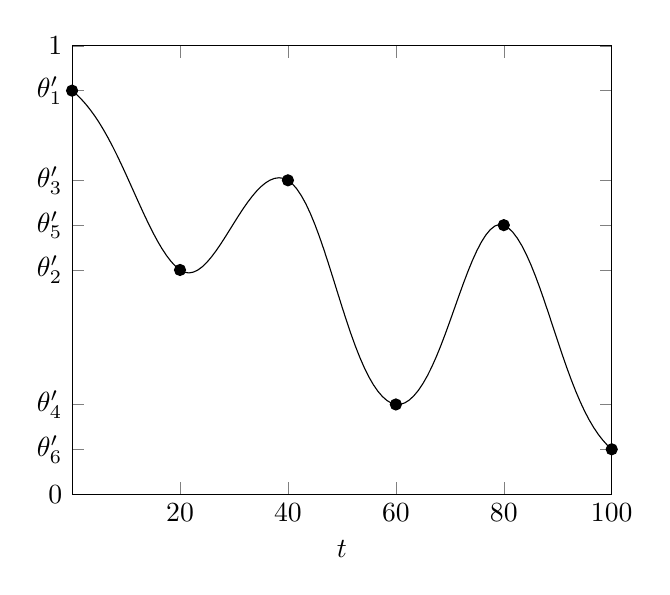
\begin{tikzpicture}
    \begin{axis}[xtick={20, 40,...,100}, ytick={0, 0.1, 0.2, 0.5, 0.6, 0.7, 0.9, 1}, yticklabels={0, $\theta_6'$, $\theta_4'$, $\theta_2'$, $\theta_5'$, $\theta_3'$, $\theta_1'$, 1}, xmin=0, xmax=100,  ymin=0, ymax=1, xlabel = $t$]

\addplot[domain=0:20] {1/(1+e^(-((2*((x-0)/(20-0))^3 - 3*((x-0)/(20-0))^2 + 1)*(2.2) + (((x-0)/(20-0))^3 - 2*((x-0)/(20-0))^2+((x-0)/(20-0)))*(0-(2.2)) + (-2*((x-0)/(20-0))^3+3*((x-0)/(20-0))^2)*(0) + (((x-0)/(20-0))^3-((x-0)/(20-0))^2)*1/2*((0-2.2) + (0.8473-0)) )))};
\addplot[domain=20:40] {1/(1+e^(-((2*((x-20)/(40-20))^3 - 3*((x-20)/(40-20))^2 + 1)*0 + (((x-20)/(40-20))^3 - 2*((x-20)/(40-20))^2+((x-20)/(40-20)))*1/2*( (0.8473-0) + (0-(2.2)))+ (-2*((x-20)/(40-20))^3+3*((x-20)/(40-20))^2)*(0.8473) + (((x-20)/(40-20))^3-((x-20)/(40-20))^2)*1/2*((0.8473-0) + (-(1.3863)-0.8473)) )))};
\addplot[domain=40:60] {1/(1+e^(-((2*((x-40)/(60-40))^3 - 3*((x-40)/(60-40))^2 + 1)*0.8473 + (((x-40)/(60-40))^3 - 2*((x-40)/(60-40))^2+((x-40)/(60-40)))*1/2*( (-(1.3863)-0.8473) + (0.8473-0))+ (-2*((x-40)/(60-40))^3+3*((x-40)/(60-40))^2)*(-(1.3863)) + (((x-40)/(60-40))^3-((x-40)/(60-40))^2)*1/2*((-(1.3863)-0.8473) + (0.4054--(1.3863))) )))};
\addplot[domain=60:80] {1/(1+e^(-((2*((x-60)/(80-60))^3 - 3*((x-60)/(80-60))^2 + 1)*-(1.3863) + (((x-60)/(80-60))^3 - 2*((x-60)/(80-60))^2+((x-60)/(80-60)))*1/2*( (0.4054--(1.3863)) + (-(1.3863)-0.8473))+ (-2*((x-60)/(80-60))^3+3*((x-60)/(80-60))^2)*(0.4054) + (((x-60)/(80-60))^3-((x-60)/(80-60))^2)*1/2*((0.4054--(1.3863)) + (-2.1972-0.4054)) )))};
\addplot[domain=80:100] {1/(1+e^(-((2*((x-80)/(100-80))^3 - 3*((x-80)/(100-80))^2 + 1)*0.4054 + (((x-80)/(100-80))^3 - 2*((x-80)/(100-80))^2+((x-80)/(100-80)))*1/2*( (-2.1972-0.4054) + (0.4054--(1.3863)))+ (-2*((x-80)/(100-80))^3+3*((x-80)/(100-80))^2)*(-2.1972) + (((x-80)/(100-80))^3-((x-80)/(100-80))^2)*1/2*((-2.1972-0.4054) + (0.2-2.1972)) )))};
\addplot[mark=*] coordinates {(0,0.9)};
\addplot[mark=*] coordinates {(20,0.5)};
\addplot[mark=*] coordinates {(40,0.7)};
\addplot[mark=*] coordinates {(60,0.2)};
\addplot[mark=*] coordinates {(100,0.1)};
\addplot[mark=*] coordinates {(80,0.6)};
\end{axis}
\end{tikzpicture}
}
\end{figure}



\item The fraction is determined by a neural network. 
\end{enumerate}    

